\documentclass[draft,12pt]{article}
\usepackage[margin=1.2in]{geometry}
\usepackage{color}
\usepackage{graphicx}
\usepackage{url}
\usepackage{wrapfig}
\usepackage{amsmath}
\usepackage{amssymb}
\usepackage[round]{natbib}
\bibliographystyle{evolution}
\usepackage[usenames,dvipsnames,svgnames,table]{xcolor}

\newcommand{\citex}{\textcolor{red}{\textbf{(CITE)}}}

%\bibliographystyle{abbrvnat}
%\setcitestyle{authoryear,open={(},close={)}}
\usepackage[innercaption]{sidecap} % side captions
\sidecaptionvpos{figure}{c}

\begin{document}

\title{Project Narrative: The genetic archaeology of maize breeding: identifying useful diversity through historical pedigree reconstruction}
\author{}
\date{}
\maketitle

\section*{Rationale and Significance}
\label{sec:rationale}

Maize is a natural resource of fundamental national importance, vital for food, livestock feed, and fuel production.
Maize is also the most valuable field crop in the United States, with production values at greater than \$50 billion dollars every year since 2010 \citep{usdanass}. 

But while maize yields have increased over the last several decades, the rate of gain falls short of projected needs in the near future \citep{grassini2013distinguishing}.
Even under stable climatic conditions, current rates of maize improvement are insufficient to meet requirements of population growth over the next 30 years \citep{ray2013yield}; in  addition to requirements in terms of food and animal feed, worldwide ethanol use is projected to increase 40\% within just the next decade \citep{usdalong}.
%could be convinced to drop the ethanol comment

Changing climatic conditions, however, will likely further challenge our ability to meet needed yield gains. 
Historical analyses suggests that climate change over the last 30 years has already dramatically impacted maize yields worldwide, retarding gains from breeding and management \citep{Lobell2011}.
Moreover, predicted temperature increases will increase volatility in yield across the U.S. and may even decrease future yields \citep{urban2012projected}, with some models suggesting a change of even 1$^{\circ}$C could negatively impact yields by as much as 17\% \citep{lobell2003climate}; more dire warnings suggest that U.S. maize yields could drop 30-46\% below current levels by the end of the century \citep{schlenker2009nonlinear}.
Substantial efforts will clearly be needed to preserve U.S. maize production and increase or maintain yields.  

Much of the historical gains in maize yield can be directly attributed to breeding efforts \citep{Duvick1992, duvick2005genetic}, and \textbf{ breeding must remain of central importance in order to meet increased yield demands}.  
Breeding is also of key importance in adapting maize to the challenges of changing climates \citep{Troyer2004a}, with recent models suggesting that efficient use of extant adaptive diversity in maize could significantly ameliorate the effects of climate change \citep{butler2013adaptation}.   

\subsection*{Diversity loss threatens breeding gains}

Breeding, and adaptation in general, relies critically on the availability of genetic diversity. 
This is best represented mathematically by JL Lush's famous ``breeder's equation'' $R=\frac{V_A}{V_P}s$, showing that adaptation --- the response to selection $R$ --- depends not only on the strength of selection $s$ but also directly on the amount of heritable genetic variation $V_A$ for the trait of interest \citep{kelly2011breeder}. 
The advent of modern hybrid maize breeding, the development of distinct breeding pools and the winnowing of inbreds from individual breeding programs has led to a marked decrease in genetic diversity. 
Analyzing genotypes of more than 4000 public and recently released private lines, we recently showed that the diversity available to maize breeders in current germplasm is less than half what it was in before 1950 (Figure \ref{fig:diversity}). 
With decreasing diversity available for breeding decreasing yield gains are a mathematical certainty. 
%over the top?

\begin{SCfigure}[][t]
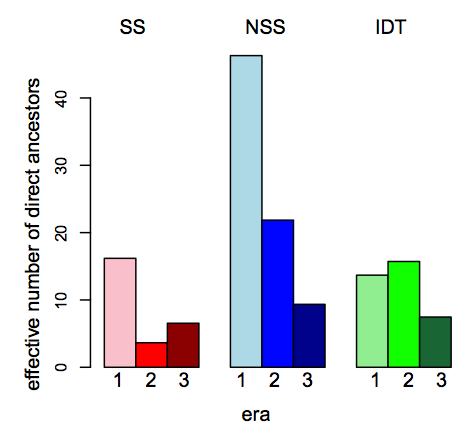
\includegraphics[width=0.5\linewidth]{joost_diversity.png}
\caption{Changes in genetic diversity (represented as the effective number of ancestors) of the three primary maize heterotic groups (SS: stiff-stalk; NSS: non-stiff-stalk; IDT: iodent). Inbreds are divided into eras representing different time periods: 1:1930-1950; 2:1950-1980; 3:1985-1992. Figure from \citet{van2012historical}.} 
\label{fig:diversity}
\end{SCfigure}

While open-pollinated varieties and exotic inbred lines represent a viable source of new diversity, these have been only sparingly used in the private sector due to their poor agronomic performance, photoperiod sensitivity, and the necessary generations of back-crossing to adapted lines required to incorporate useful alleles into high-performing temperate germplasm \citep{goodman1999broadening}.
In contrast, older U.S. inbred lines, though lower-yielding than their contemporaries, harbor novel genetic diversity of potential use for breeding but are already adapted to the U.S. cornbelt.  
For example, a recent phenotypic evaluation identified several older inbreds as sources of useful variation for drought and heat tolerance \citep{chen2012characterization} and our own population genetic analysis identified a number of older inbreds enriched for underutilized adaptive alleles (Figure \ref{fig:wf9}).

\begin{SCfigure}
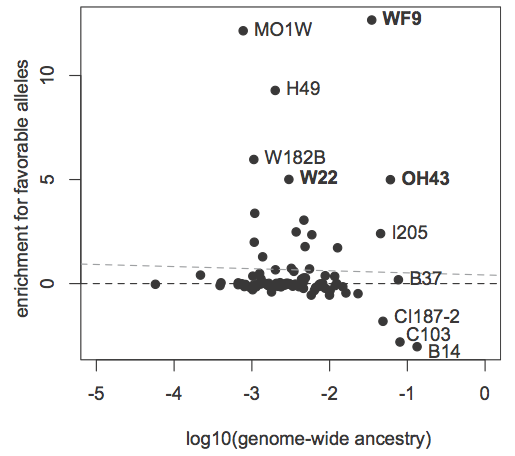
\includegraphics[width=0.5\linewidth]{joost_wf9.png}
\caption{Enrichment (defined as the log probability ratio with respect to control loci) of favorable alleles in older (era 1) inbreds as a function of their average ancestral contribution to modern (era 3) lines. The black dotted line represents the 0 horizontal, and the gray dotted line the regression  with slope −0.1). Inbred names are shown for lines with log probability ratios higher than 4 or ancestry proportion above 0.03. Labels in boldface mark breeding lines of known historic popularity. Figure from \citet{van2012historical}.} 
\label{fig:wf9}
\end{SCfigure}

\subsection*{Lack of public resources limits use of diverse germplasm}

Breeders will not blindly incorporate older material into their populations, however.  
Perhaps the most important piece of information required to effectively utilize older germplasm is pedigree.
Pedigree data immediately gives a breeder information on crosses likely to produce higher yields due to heterosis, and often provides additional utility in identifying likely maturity (flowering time) and other agronomic characteristics. 
Combined with phenotype data, pedigree information can even be used to predict phenotype even in the absence of genotype \citep{piepho2008blup} and pedigree-based methods for identifying useful diversity have already been patented by industry \citep{sebastian1995method}.

While private industry may in many cases have detailed records of their own breeding material, the vast majority of private germplasm is founded on $20^{th}$ century public breeding lines \citep{nelson2008molecular}.

Unfortunately, pedigree data for most U.S. maize inbreds is unavailable to most breeders. 
For example, of the over 45,000 worldwide inbreds in the USDA Germplasm Resources Information Network, only some 34,000 have some amount of ancestry determined, and much of this information is incomplete.
If we look at available germplasm only, that number shrinks to 2931 accessions with any available ancestry information.
While there are published compilations of germplasm, these are far from complete:  \citet{gerdes1993compilation}, for example, contains complete pedigree data for less than \textcolor{red}{XXX}\% of the germplasm in the USDA database.
%I actually don't know this actual figure - but would presume on the order of 10% or less (fuzzy matches).
Moreover, what ancestry information that is available is not in electronic form nor easily accessible in any single resource.  
Instead, historical pedigree information exists primarily in the minutes of breeding committees, old breeding program books, and other hard-copy sources with limited distribution.  

{We propose to  generate an open-source database of public maize pedigrees and genotypes and use this resource to identify genotypic and phenotypic diversity of high utility in advancing maize breeding.}
%this reads too long, efforts to shorten are welcome.
Given the importance of maize to U.S. agriculture, this proposal clearly aligns with the USDA AFRI program priorities of ``Plant Breeding for Agricultural Production.''  
Our proposal will develop tools to accelerate breeding by allowing breeders to more quickly identify useful inbreds, and our application of population and quantitative genetic methods will identify specific genetic and phenotypic diversity of potential use for future breeding.  
%do we say something about ``Development and application of tools to predict phenotype from genotype to accelerate breeding of finished varieties;'' (from the RFA)??

\section*{Introduction}
\label{sec:introduction}

%a. Introduction
%Include a clear statement of the long-term goal(s) and supporting objectives of the proposed project. Summarize the body of knowledge or past activities that substantiate the need for the proposed project. Describe ongoing or recently completed activities significant to the proposed project including the work of key project personnel.


\subsection*{Maize breeding}
Maize has undergone dramatic phenotypic and genetic changes since its domestication and subsequent spread through North and South America \citep{daFonseca:2015ey,Doebley:2004ce}. More recently, beginning in the mid-20$^{th}$ century, the intensification of maize breeding efforts has lead to subtler but equally important changes including increasing yields and improved agronomic traits such as leaf angle and density tolerance \citep{duvick2005contribution}. 

Maize is  a self-compatible crop, and modern breeding programs (post-1960) take advantage of self-fertilization (or now double-haploid technology) to create homozygous inbred lines. 
Distinct inbreds are maintained in separate breeding pools or heterotic groups.
The most important heterotic groups among U.S. public germplasm are the ``stiff stalk'', ``non-stiff stalk'', and ``iodent'' (Figure \ref{fig:diversity}).
Inbred lines from separate breeding pools are then crossed to make hybrid progeny.  
These hybrids often display heterosis, meaning that yield and associated traits of the hybrid are superior to  either inbred parent \citep{Springer:2007bj}.  
Inbreds capable of producing high-yielding, heterotic offspring are said to have good ``combining ability'', and are recycled in their respective breeding pools.
Inbreds that form less desirable combinations are usually discarded from the breeding pool. 
Useful inbreds within a group are crossed with each other, and their segregating progeny evaluated and self-fertilized to create new inbreds. 
Maintaining this system for propagation of inbred lines and hybridizing inbreds for evaluating production traits has worked well for many decades, but there is growing reason for concern that this method may need a genetic boost. 

\subsection*{Decelerating yield gains} 

Maize yields have steadily increased since the advent of hybrid breeding in the 1930's.
But linear increases necessarily mean a decrease in relative gain, and projections suggest that current trends are unlikely to meet future yield goals \citep{grassini2013distinguishing}. 
Of even greater concern is the possibility that the rate of gain may actually be decreasing (Figure \ref{fig:piecewise}).
While some of these yield trends are undoubtedly related to changing management practices, much of the change is indeed due to breeding \citep{Duvick:2001fy}, and current rates of yield gain are lower than historical trends even after correcting for nitrogen fertilizer inputs (data not shown). 
%i don't want to try to explain the inflection point figure. do we just cite wherever you got the N2 data from?  do we include but change the graph? do we not even mention? ideas?

\begin{SCfigure}
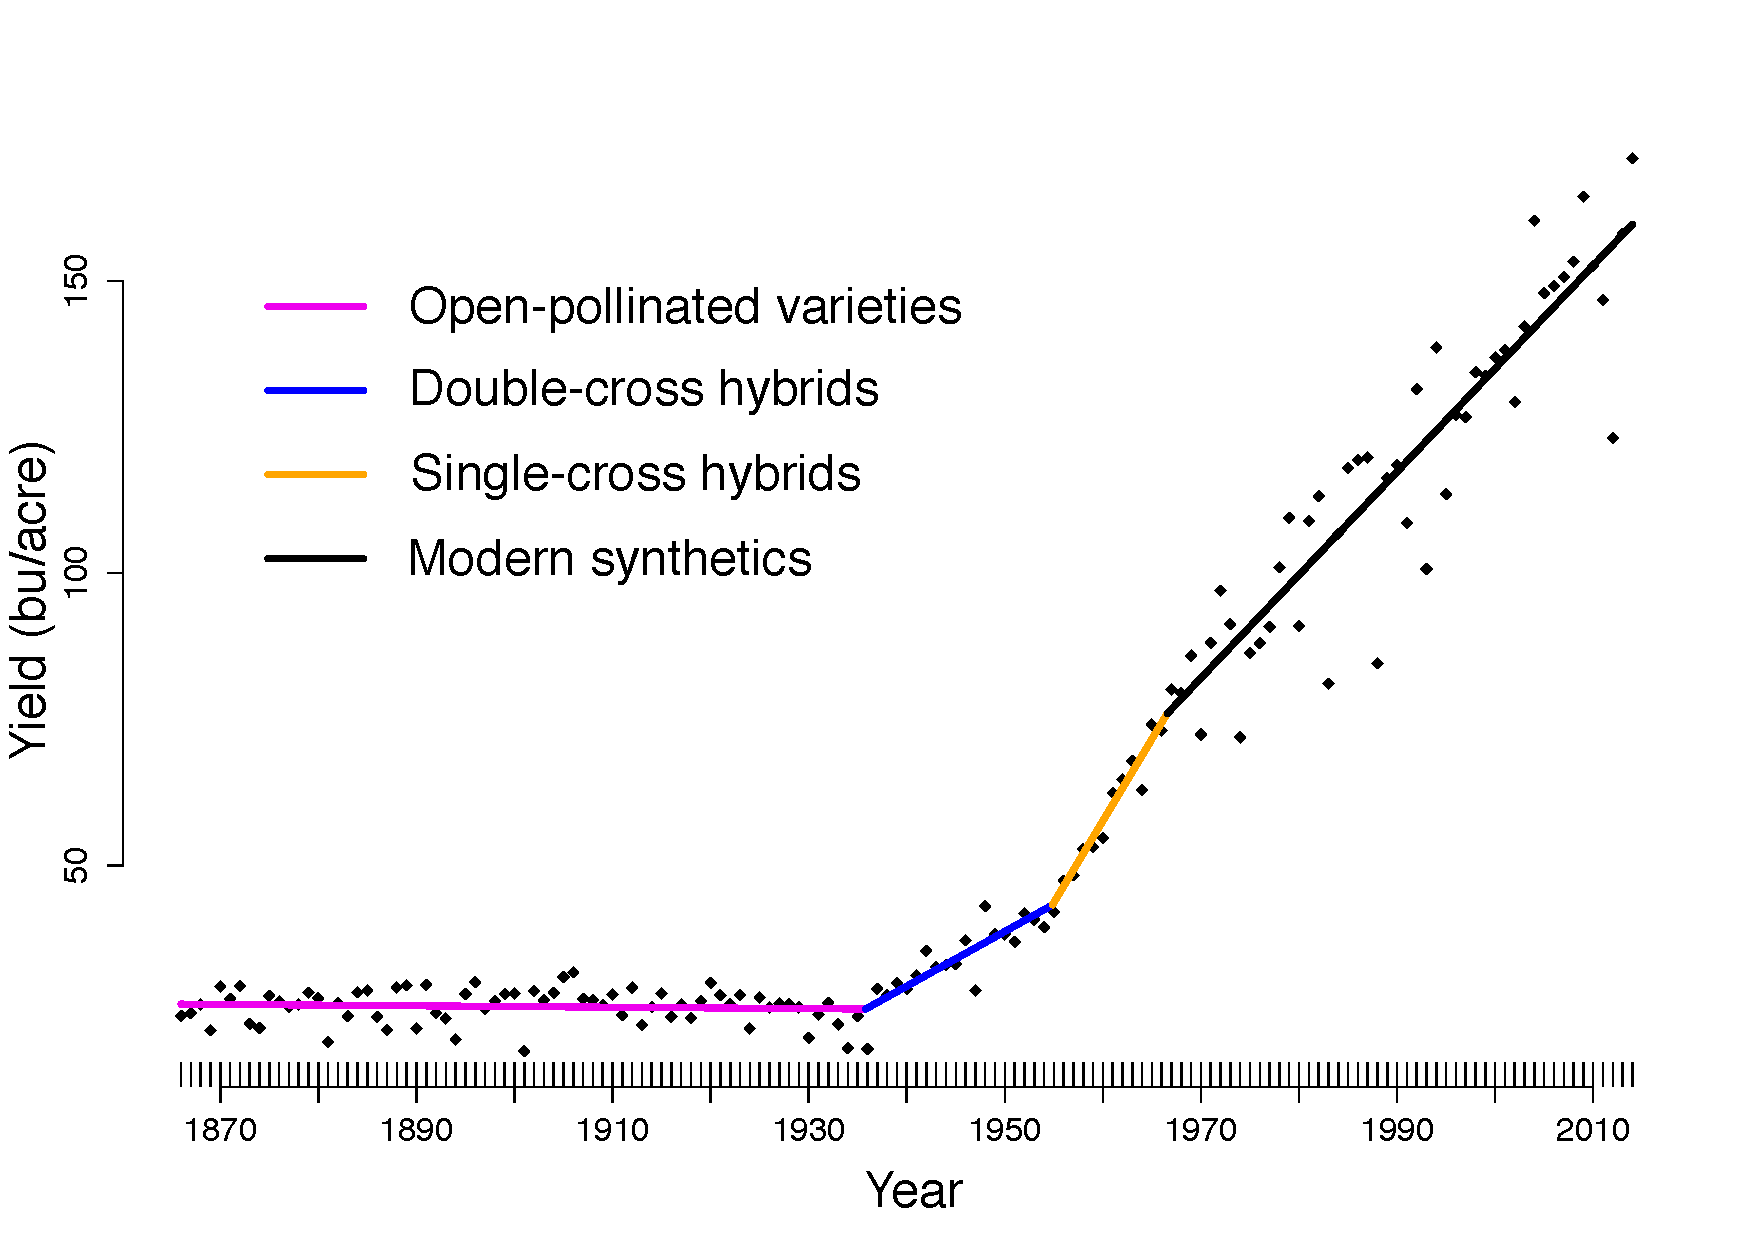
\includegraphics[width=0.6\linewidth]{yield.pdf}
\caption{Piecewise regressions of time against total yield through the four eras of modern maize breeding. Colors represent distinct eras of maize breeding that roughly correspond to the eras  referred to in Figure \ref{fig:diversity}.} 
\label{fig:piecewise}
\end{SCfigure}
 
% * <jholland@ncsu.edu> 2015-03-30T19:07:13.871Z:
%
%  the reaction by breeders to this is likely to be: such lines are dropped for good reason, and breeding gains may require some loss of diversity, since much of diversity is not favorable. i wonder if the objective needs to be something more like identifying this lost diversity is important assuming that SOME of those alleles are useful and were lost due to drift, negative hitchiking, or whatever. I bet there are many of those alleles that no breeder wants to see again, inbred performance is just so much better now than 50 years ago.

%\begin{figure}[ht]
%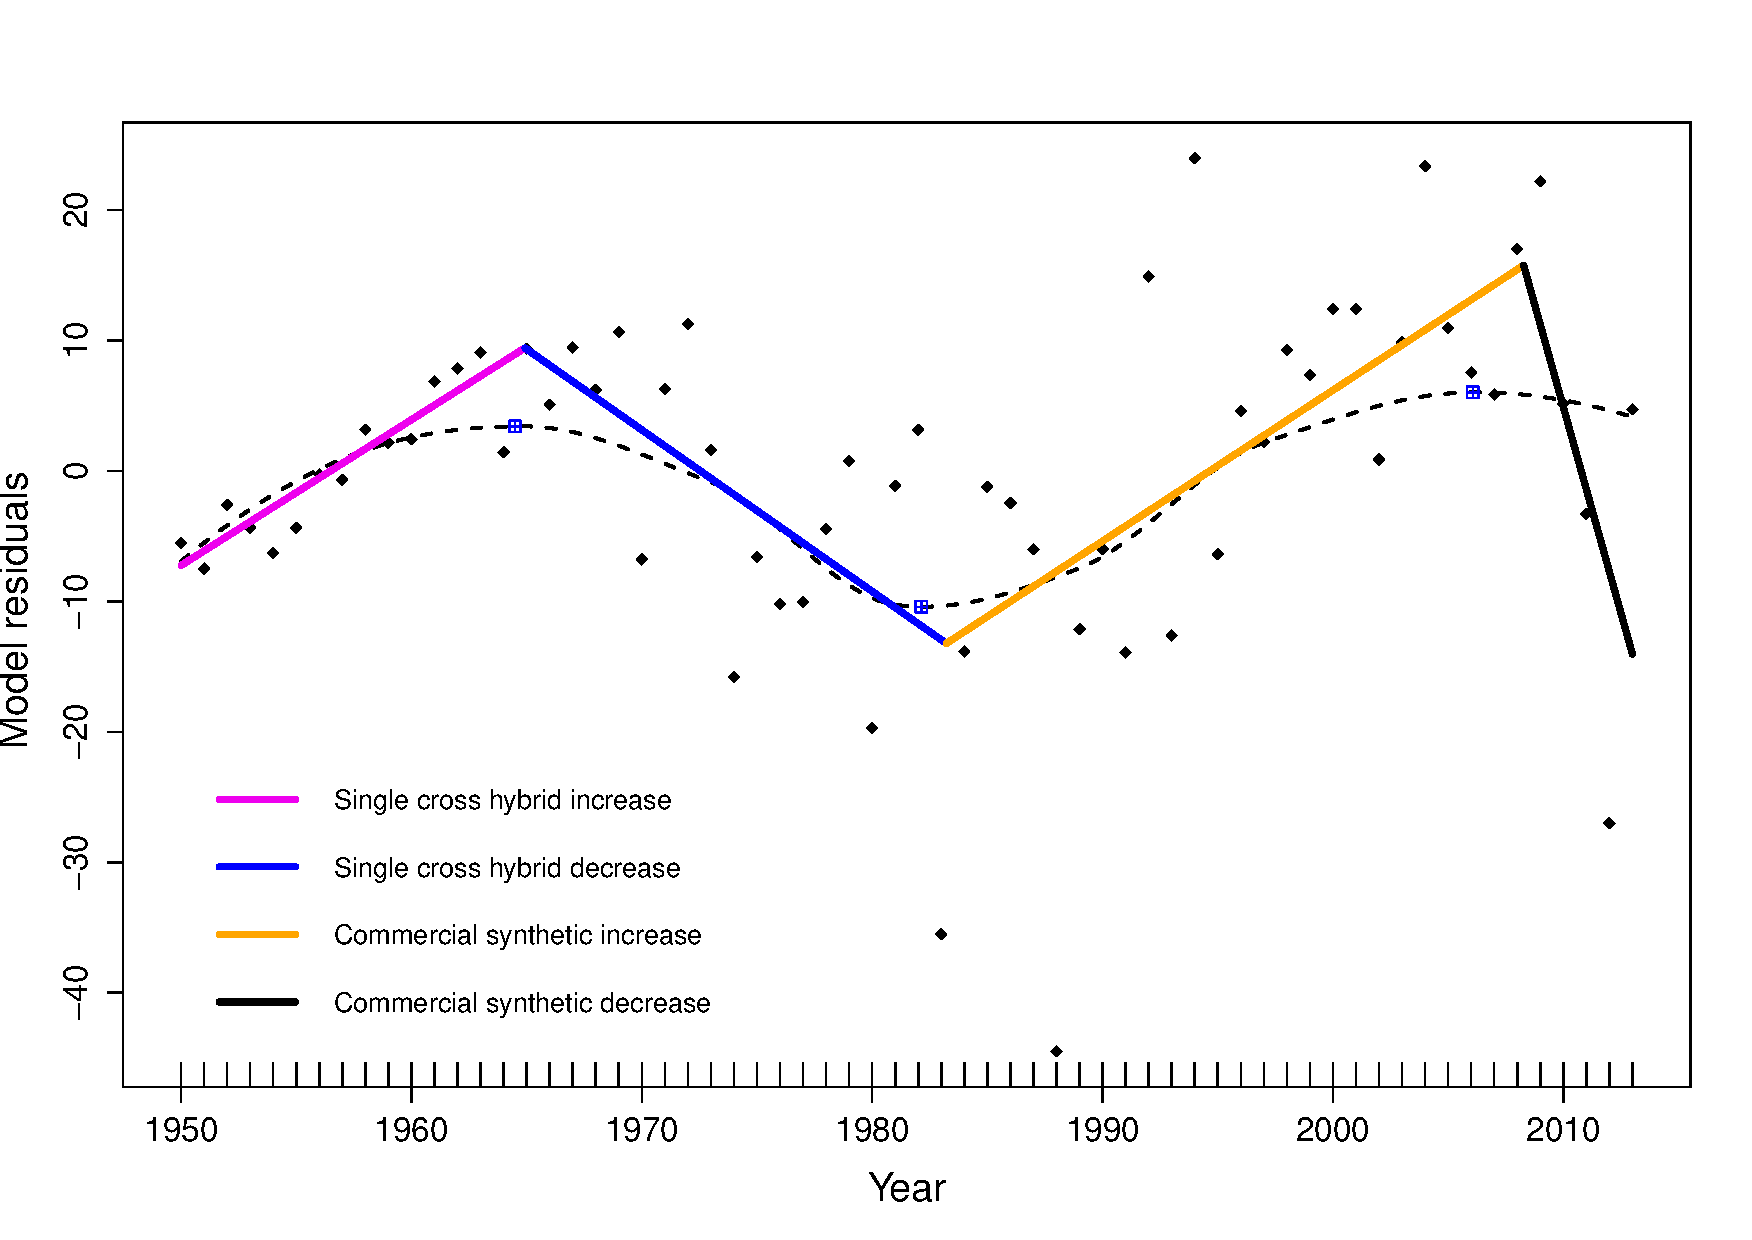
\includegraphics[width=1.0\linewidth]{inflection_point.pdf}
%\caption{Model residuals after removing the effect of nitrogen from Figure \ref{fig:piecewise}, with inlection points (blue squares) and piecewise regressions showing the possible points allelic gains and losses through time.} 
%\label{fig:inflection}
%\end{figure}

\subsection*{Decreasing diversity} 

As selection progresses within a breeding program, inbred lines with poor performance are generally discarded, leading to a decreased effective population size ($N_e$) of the breeding pools.
Response to selection $R$ depends both on the strength of selection $s$ and the narrow-sense heritability of a trait, which is the ratio of the additive genetic variance $V_A$ to the phenotypic variance $V_P$ \citep{kelly2011breeder}:
\begin{align*}
R=\frac{V_A}{V_P}s
\end{align*}
The expected additive genetic variance of traits between relatives, in turn, depends on the effective population size $N_e$ as well as the mutational variance per generation ${\sigma}_m^2$ \citep{whitlock1999neutral}:
\begin{align*}
E[V_a] = 4N_e {\sigma}_m^2
\end{align*}
A reduction in $N_e$ thus inherently leads to a reduced response to  selection, leading to diminishing returns on yield unless new diversity is brought back into breeding pools.
Evidence from the Iowa Reciprocal Recurrent Selection breeding program suggests these concerns are valid (Figure \ref{fig:trends}), as yield gains plateau over time \citep{rouse2003selection} concomitant with continued declines in genetic diversity \citep{Gerke:2013tw}.
\textbf{ Decreasing $N_e$ (Figure \ref{fig:diversity}) in U.S. cornbelt germplasm risks our ability to maintain or increase rates of genetic gain in yield.} 
%stop here? mention anything about importance of Iowa RRS?


%\begin{figure}[ht]
%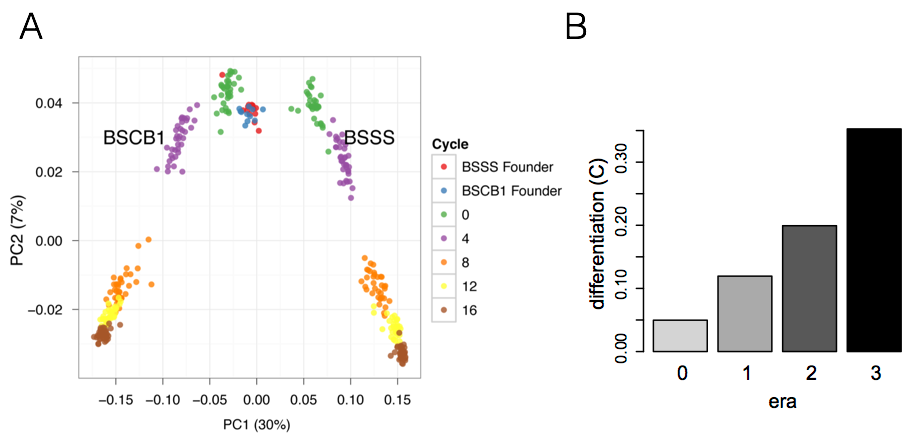
\includegraphics[width=\linewidth]{joostgerke.png}
%\caption{Changes in diversity and population structure during maize breeding.  
%A) Principal component analysis of genotypes from the Iowa Reciprocal Recurrent Selection population. The first eignevector represents divergence between the two heterotic pools, and the second divergence over time within each pool. Figure from \citet{Gerke:2013tw}. 
%B) Population structure --- quantified by the differentiation statistic C --- over time across all U.S. public inbreds. Eras represent time periods in Fig. \ref{fig:diversity}; figure is from \citep{van2012historical} } 
%\label{fig:pca}
%\end{figure}

\subsection*{A novel approach to incorporate new diversity}

Incorporating novel diversity into contemporary modern maize lines is clearly an important goal necessary to maintain and increase rates of yield gain.
While there are other public efforts to achieve this goal, like the GEM  (Germplasm Enhancement of Maize) program \citep{pollak2003history}, these  focus on incorporating exotic germplasm into U.S. materials by introgressing high quality exotic germplasm (e.g. CIMMYT lines, tropical hybrids, etc.) into well-adapted U.S. cornbelt backgrounds.
While this approach is successful at bringing in new diversity, it requires time-consuming back-crossing before it can generate lines that are of sufficient quality to incorporate into a breeding program.

\begin{wrapfigure}{R}{0.5\textwidth}
%\begin{minipage}[t]{0.5\textwidth}
%\begin{SCfigure}
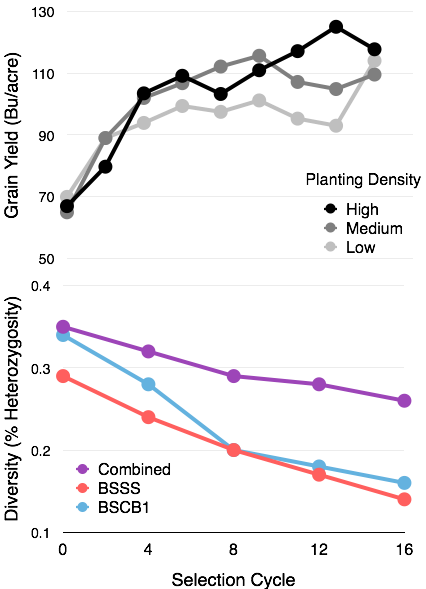
\includegraphics[width=0.5\textwidth]{BSSS.png}
\caption{Yield and genetic diversity in the Iowa Recriprocal Recurrent Selection Program across 16 cycles of selection. (Top) Grain yield at three planting densities; data are from \citet{rouse2003selection}. (Bottom) Genetic diversity of the BSSS and BSCB1 breeding pools separately and combined; data are from \citet{Gerke:2013tw}.} 
\label{fig:trends}
%\end{SCfigure}
%\end{minipage}
\end{wrapfigure}

\textbf{We propose a different approach, using pedigree and genetic data to identify underutilized cornbelt germplasm.}  
While this approach shares with projects like GEM the disadvantage that diverse material is often  agronomically inferior, it has several advantages.  
First, with sufficient information (see below), breeders may be able to learn a substantial amount about the potential utility of a line by predicting phenotype directly or understanding its relationship to known material. 
Second, in contrast to exotic germplasm, older U.S. germplasm is already reasonably well-adapted to the photoperiod and climate of the U.S., meaning it can be immediately incorporated into breeding programs.
\textcolor{red}{MORE ADVANTAGES??}

\subsection*{Identifying useful diversity}
As any breeder will attest, many old lines have fallen out of use precisely because they showed inferior agronomic performance.
%Can put in here that this is selection ON phenotypes not genotypes (as it always is with breeding) - ideally we could select on alleles 
%Current methods allow us to get at the ``adaptive alleles'' or we propose that they should even in the baddie lines
%Germplasm can be resurrected, targeted for beneficial alleles and introgressed back in
There are a number of reasons, however, why older lines may retain useful genetic diversity.
First, lines are often discarded or selected against because of poor performance for a particular trait, which does not preclude that line's utility in breeding for other traits.
For example, thanks to its combining ability, the U.S. inbred B73 quickly spread in popularity and now makes up a considerable portion of modern breeding material \citep{van2012historical}.
Yet when evaluated for drought and heat stress, B73 significantly underperformed compared to less well-utilized lines such as B76 \citep{chen2012characterization}.
Second, the contribution of older lines to modern germplasm does not necessarily reflect their genetic potential.
Our previous analysis of maize ancestry found popular lines with fewer beneficial alleles than expected given their importance to modern germplasm as well as lines with more beneficial (as defined by a steady increase in allele frequency over time) alleles than expected (Figure \ref{fig:wf9}).

\begin{itemize}
\item popgen point about alleles lost due to drift
\item previous efforts like our popgen only looked at allele frequency. this is problematic because of structure etc.
\item pedigree analysis allows improved popgen and other benefits (discuss)
\end{itemize}

\subsection*{Pedigree-based approaches to identifying useful maize germplasm}


\subsubsection*{advantage of pedigree}
\- what you can do with a pedigree

\subsubsection*{Preliminary work: pedigree records to date}
To date, we (Drs. Smith and Crosby) have gathered parentage info for over 3193 lines and originally built a large pedigree of some 700 lines (Figure \ref{fig:b73isbig}is but a small portion of this pedigree) with complete parentage information that overlaps with currently available GBS maize 2.7 data \citep{Glaubitz:2014eu}. 
\par Further work, has led to a total of 1696 records overlapping with GBS data, and we have applied the approach of allele-dropping \textcolor{red}{add in basic allele dropping schematic - and then show for some families} to some lines that feature heavily in the pedigree.

\subsubsection*{Preliminary work: allele dropping works? GBS pruning?}


\begin{figure}[ht]

\includegraphics[width=1.0\linewidth]{pedigree_poster.pdf}
\caption{Reconstructed pedigree data for the inbred line B73 that features heavily in modern germplasm.}
\label{fig:b73isbig}
\end{figure}

\paragraph{unincorporated text $->$}
Pedigrees, especially when combined with modern genomic and phenotypic trait data, are useful tools for predicting phenotype \citep{crossa2010prediction} and identifying beneficial alleles \citep{sebastian1995method}.
 that have experienced strong artificial selection across breeding pools. Examples of their application can be found with: cattle \citep{Decker:2012kd}, soybean (cite), and grape (cite). 
While private companies likely have their own pedigree databases to do exactly this, these data are private, patented, and not available to the public. 
Further, much of the pedigree information on older founder inbred maize lines sits in old volumes of Crop Science or the Agronomy Journal, experimental station technical bulletins, regional corn breeding meeting records, release sheets, or breeding books, unused and vulnerable to loss.  
The National Plant Germplasm Service (NPGS) database contains information with regards to ancestry of public maize inbred lines, much of this information is incomplete or missing (see section above). 
However, much of this ancestry information on modern maize lines  is still publicly available, only not in digital form, nor is it easily-accessible. This historical pedigree information exists in old volumes and minutes of breeding committees, old breeding program books, and other hard-copy-only sources. Here, we propose a project that will help preserve, maintain, and use this historical information with novel genomic data to better benefit future maize breeding programs.

\section*{Approach}
\label{sec:approach}
Our proposed research has three major aims in using pedigree information to detect historic shifts in allele frequencies of modern inbred maize lines.

\begin{itemize}
\item Aim 1: Digitize and curate pedigree and genotype information into a publicly available database. 
\item Aim 2: Identify adaptive alleles using a combination of pedigree and population genetic approaches.
\item Aim 3: Phenotypic and genotypic evaluation of individuals lines that feature heavily in the historical pedigree.

\end{itemize}
\subsection*{Proposed activities, methods \& feasibility}
\subsubsection*{Travel and digitization of records and agreed upon database format for all data}
The first part of our proposal aims to preserve hard-copy pedigree records by traveling to different land grant institutions by digitizing them. 
These raw data scans will then be manually translated into an agreed upon format, with numbering/naming of each line/accession agreed upon.
Dr. Kate Crosby, Dr. Taner Sen (support letter from maize GDB enclosed), senior personnel Dr. Oscar Smith, and CO-PI Dr. Bill Tracy will consult on an agreed upon standard format with which to store the raw scan of pedigree records, the phenotypic and genomic information. 
Establishing an agreed upon format in the first few months of the project will enable easy mapping of current and future genomic data formats to pedigree information.
Additionally, Dr. Kate Crosby is currently investigating the possibility of using no-SQL database without formal schemas specified \textit{a priori} (graph databases) to be able handle queries with respect to mapped genomic data, extended ancestry, and phenotypic data, along with new visualization tools \citep{ParejaTobes:2015bf}.

\subsubsection*{Genotyping of lines that feature heavily in historical pedigree information}
Undoubtedly, there will be information obtained from historical pedigree information on lines that do not have any genomic data available for them. 
In such cases (where germplasm is available), we intend to use genotype-by-sequencing (GBS) \citep{Elshire:2011ha} as a cost-efficient platform \citep{Glaubitz:2014eu} to obtain high-coverage and density of SNPs  for these lines, with markers aligned to the newest maize reference genome (currently B73 v. 3). 

\subsubsection*{Project 1 for student 1: understanding the dynamics of selection through time with allele-dropping and pedigree}
In the section above we mention that certain maize lines feature heavily in the historic pedigree. For example, in the public pedigree B73 features heavily as a parent to many ancestors of current inbred lines (Figure \ref{fig:b73isbig}). 




The first masters student to be supervised by Dr. James Holland (NC State) will, with the cooperation of Dr. William Tracy, Dr. Sherry Flint-Garcia, Dr. Oscar Smith, and the post-doc Dr. Kate Crosby use the information gathered during the first year to identify these historically important lines. 
Many small pedigrees will be constructed from lines identified as having many inbred ``progeny''. 
This student will then identify distorted segregation at all heterozygous loci (using GBS markers) within and across these many small pedigrees (Figure \ref{fig:alleledrop}), this is known as \textbf{``allele-dropping''}. 
It is a simple Mendelian approach to identifying traces of selection by directly accounting for ancestry, and without the worry of having to account for shared population structure (as in modern population genomics approaches). 
If we can identify the uni-directional shift of a given allele across many of these small pedigrees at a set locus, this would indicate selection. 

The student would also be responsible for simulating allele frequency change under neutral processes (genetic drift). The approach would be similar to that used in \citep{Gerke:2013tw}, to evaluate at which loci adaptive (by breeders) or neutral forces have shaped the current allelic diversity of the overall modern breeding population. 
Should loci be identified as having uni-directionally shifted through time across many of these small pedigrees, we would compare this to our findings in project 2 (see next section \textbf{project 2}).

\begin{figure}[p]
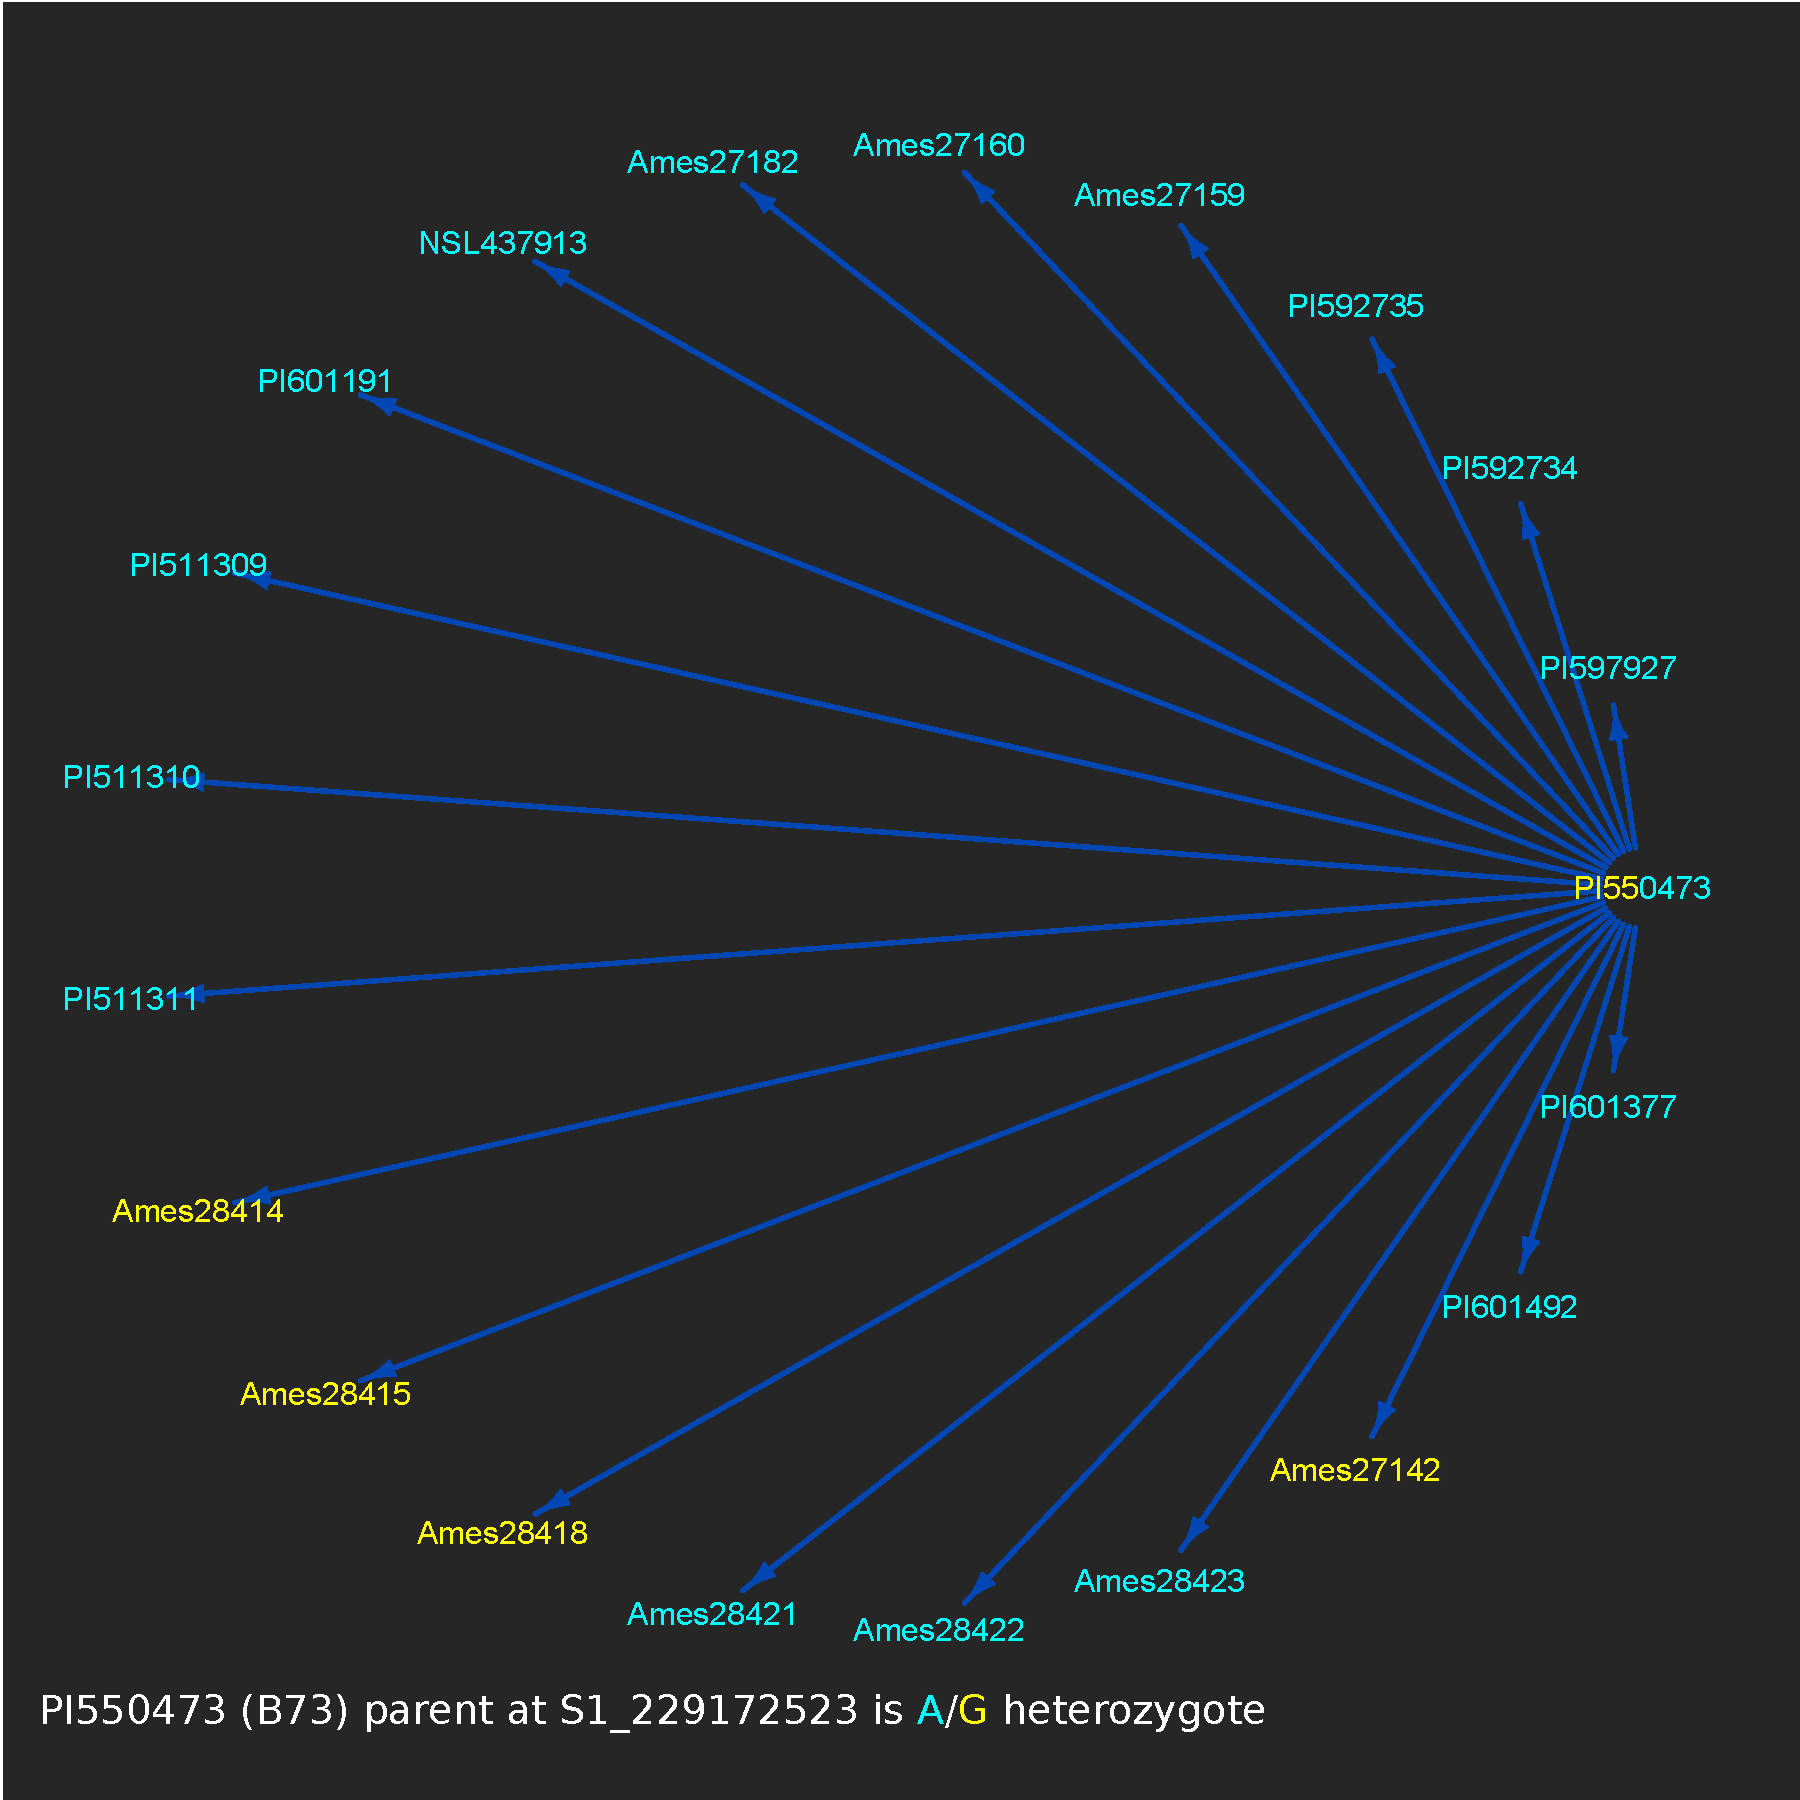
\includegraphics[width=1.0\linewidth]{Pruned.pdf}
\caption{B73 (also known as PI550473 by NPGS and a number of its inbred progeny) is heterozygous at 379 loci out of over 954,000 loci with GBS markers). The blue labels represent which inbred progeny obtained the A allele, whereas the yellow labels indicate the progeny that have obtained the G allele at a particular locus. \textbf{NB: the other parent of these lines is not indicated for simplicity}.}
\label{fig:alleledrop}
\end{figure}






\subsubsection*{Project 2 for student 2: novel population genomics approaches to project current phenotypes back in time}
%Probably should explain Qst and Fst more? Latta's intro is clear on this problem.
Novel population genomic approaches described in \cite{Berg:2014bs} propose the idea of using a technique analogous to $Q_{ST}$- $F_{ST}$ approaches popularized in the 1990s \citep{Latta:1998ek,  McKay:2002wi}, but applied to large numbers of SNP marker hits from Genome-Wide-Association-Studies (GWAS). 
GWAS hits have typically fallen short in explaining much of variation in quantitative characters \citep{Rockman:2011ej}, with only a small portion of GWAS hits associated with or close to a quantitative trait locus (QTL) of large effect. 
This lack of signal in GWAS hits may be due to the polygenic nature of many traits, with the genetic basis of each trait explained by many loci of small effect(s). 

With polygenic signals and their effects scattered throughout the genome, these become difficult to detect and interpret with conventional statistical methods. 
In order to be able to detect these weak signals, \cite{Berg:2014bs} compare the dispersion of GWAS hits, and their effect sizes (in different environments or time periods), to random sets of SNPs (from the same time), and look for a correlated shift in alleles associated with traits of interest in each divergent environment (or, in our case time period).
%-Do I provide Qx statistic here?
Dr. Randall Wisser's student will be responsible for performing this analysis on lines deemed to be of interest from both periods (likely those founder parents and their progeny or later generation ancestors). 
%I know Qx accounts for structure - but I think looking at inter-familial and extra-familial will be cool (different covariance matrices for sure.
The student will then grow out these lines as a way of verifying that the SNPs in earlier founder lines shared with later familial and extra-familial lines express the expected additive phenotype for production traits of interest. 
By combining population genetics with quantitative 



\subsection*{Expected outcomes \& Utility of results}

\subsubsection*{A user friendly, open database}

Our first expected deliverable is an open public pedigree database to be hosted on maize GDB for the long term future. Users will be able to contribute and revise incomplete information, with the goal of establishing a nearly complete public pedigree of maize inbred lines. \textbf{To our knowledge, this will be one of the first public crop databases of its kind (with lines having genomic and phenotypic data mapped onto entries).}

Ensuring data, code, and script are open-access or open-source (freely available to the public) is important for critique, debate, and dialogue in science. Dr. Ross-Ibarra has a long track record of ensuring openness with his science, data, and code. Throughout this project, both Dr. Ross-Ibarra and Dr. Crosby will endeavour to ensure that code and data are available via repositories such as github, figshare, maize GDB, and iPlant.

\subsubsection*{From quantitative genetics to population genetics and back again}
One of the drawbacks of using QTL mapping and traditional GWAS studies to identify adaptive alleles/loci is that many alleles may not be identified due to the diffuse polygenic signal of many traits \cite{Rockman:2011ej, Berg:2014bs}. 
Here we propose the first study to look for correlated allele shifts (thought to be associated with production traits) in lines from temporally (not spatially) different environments using a population genomics approach.
%The next paragraph may just be dropped, I know you said crosses are unlikely, and looking at Randy's facilities, I bet we won't be able to look at these - it is drool worthy for me. Popgen signal of quantgen, ground truthed with hard quantgen
\par What makes this study particularly unique is that germplasm of older lines can be ``resurrected'' similar to approaches used in resurrection selection studies for climate adaptation \cite{Franks:2007be}, but here we will have ample genomic data for sets of temporally differentiated lines. 
We will then be able to assess the $V_{A}$ traits based on estimated effect sizes of individual alleles, and the corresponding $V_{A}$ in the phenotype within families.
%I actually really like this Va (GWAS Snps breeding values from Berg Coop) ~ Va (trad) comparison. My inclination is that we won't find much - but if we do or even if we don't it's a PNAS paper at least (This is contingent on being able to assess crosses - no crosses - no real trad Va) and we ixnay).
%No crosses between different eras within lines? Would be cool - can get at phenotypes/genotypes AND alleles. 

 
%- identification of ghost ancestors? \cite{Gravel}

\subsubsection*{Parameterizing heterozygous error rates of GBS}
%Basically just AA*AA cannot produce an AC inbred progeny (unless mutation), but with GBS this is an error - and I think we'll get good estimates of this. It's a side a advantage, but it's a Bioinformatics note if it's done across an entire pedigree.
A final, perhaps seemingly small advantage is that pedigrees with the allele-dropping approach will be able to help identify heterozygous error rates in GBS (see section below). As inbred lines produced from a cross between two divergent parental inbreds should show very low residual heterozygosity (at cycle 6 there should be $<$ 1\%).
This low overall residual heterozygous value in inbred progeny should be approximately equal to that of the inbred parents (as they are all inbreds produced in the same way). 
Further, only divergent homozygous loci in the parents may be heterozygous in the offspring.
Thus, any heterozygous loci in the offspring will be evaluated against loci in the parents. If the parental loci are not divergent (different) then this is an erroneous call in the offspring.  

\subsection*{Means of analysis/interpretation}
Dr. Randall Wisser has agreed to provide plot space for growing up germplasm of lines disproportionately present in the pedigree that have phenotypic data affiliated with their release sheets or with NPGS, i.e. drought resistance, heavy-metal tolerance, disease resistance, etc (see attached facilities sheet at the University of Delaware) . 
The main purpose of this grow-out is to ground truth both the information from release sheets and compare this to the suppositions gained from \citep{Berg:2014bs}, with lines that appear to harbor alleles that contribute to production traits (see section above).
Dr. Sherry Flint-Garcia has offered to aid Dr. James Holland student with obtaining germplasm and information at the USDA in Columbia, Missouri on lines deemed to be have been of great importance to the modern maize breeding by Dr. Oscar Smith and Dr. William Tracy (the ``C.I. inbreds''). 
Dr. Oscar Smith and Dr. William Tracy are experts with respect to maize breeding and pedigrees, and will quickly (due to their extensive experience) be able to validate information pertaining to parentage of inbred lines.



\subsection*{Limitations \& Prospective pitfalls}
While we are very optimistic about the prospect of obtaining accurate pedigree information from these various institutions the nature of corn-breeding and record keeping of corn-breeding can be nebulous. 
Ideally, we would be able to accurately count the number of meioses in the total pedigree, in each heterotic group, down to each line; thus, retracing the complete ancestry of a given contemporary inbred. 
However, in many cases, it may not have been noted at which point in a breeding program a line was bulked at, nor on occasion which lines were used in recycling an inbred when seed was exhausted. 
For instance, a record from NPGS may indicate that a line was bulked and stored at cycle 6, or it may have been bulked and stored at cycle 4. As a ballpark figure, a ``cycle 6 inbred'' means that germplasm from that line is 99\% homozygous at all locus pairs. 
Meaning that if this inbred is selfed further, not much changes with respect to levels of homozygosity nor heterozygosity (as recombination via selfing is ineffective beyond this point).  
Thus, so long as an inbred is at or beyond cycle 6, it will be kept, but inbreds before this period shall be discarded.
To ensure that historical records of inbred lines are isolated at cycle 6 and beyond we will investigate the level of heterozygosity in each of these lines with GBS data relative to the total amount of missing data in an individual line. Within a reasonable confidence limit most lines should show a very small portion of heterozygous loci even with GBS markers (known to have a high rate of error in undercalling heterozygous). 
Historical pedigree records and other information on old lines may be available, but the germplasm from these old lines may simply not be available (genomic data will not be able to be mapped onto these lines. 
Currently, we know that approximately 12.9\% of germplasm from NPGS for which we have parentage information is not available. Undoubtedly, as we add more records from breeding books, we expect a similar level of unavailability of germplasm.  
In such cases, we would seek available germplasm from the next nearest relatives according to historical information, and genotype those accessions. 


\subsection*{Hazards to personnel}
There will be car/air travel required by Dr. James Holland's masters student, CO-PI Dr. William Tracy, and the post-doc Dr. Kate Crosby) to the different land grant institutions. 
This travel is required for obtaining pedigree records from each land grant institution's library during year 1 of the proposed three year grant. Air travel will likely be necessary for the students and the post-doc to travel to a conference (most likely the Maize Genetics conference in 2016 or 2017) to present their results to the maize community at large. 
Travel is likely the most dangerous activity that any personnel will experience for the duration of this project, so we will take steps to ensure that all participants have travel insurance and benefits during these periods, and
this is reflected in our current budget. 


\subsection*{Timeline}
A graphical timeline of our three-year proposal is presented below. %Holding back till hear from Holland

The first year will be spent traveling and gathering and digitizing pedigree records at land-grant institutions that have been identified by CO-PI Dr. William Tracy (one of two authors of the most authoritative public guide on the pedigrees of maize inbred lines to date) and senior personnel Dr. Oscar Smith (recently retired senior corn breeder who spent 30 + years with Dupont Pioneer) as having had breeding programs, but where records have not been digitized or made widely available. 

Dr. William Tracy and Dr. James Holland's masters student will largely be responsible for traveling to and scanning hard-copy records into digital format. Dr. William Tracy has committed to obtaining records from the University of Wisconsin, University of Nebraska, and will also visit the University of Florida. 
Dr. James Holland's student will be responsible for the breeding records at North Carolina State University, Virgina Tech, and the inbred records housed at the USDA at the University of Missouri. We estimate that this should take no longer than a few weeks at each institution with the first student or CO-PI. 

The scanned digital records must then be translated into a usable data format for further analysis with NGS or phenotype data. At worst, this will involve the student, CO-PI (Holland or Tracy) or the postdoc (Crosby), physically reading and translating each of the scanned papers, and this could take several months to the entire first year depending on volume of records. 
Dr. Kate Crosby with assistance from Dr. Oscar Smith, Dr. William Tracy, with cooperation from Dr. Taner Zen will be responsible for ensuring a consistent data format for hosting on maize GDB.

At the start of the second year, any inbred line that is disproportionately present in the pedigree with available germplasm, but that has no to little genetic information on it will be genotyped using the GBS platform. 

Dr. Randall Wisser's student will then start and over a period of 3-6 months will learn the population genomics approach presented in \citep{Berg:2014bs}, as well as identify and incorporate phenotypic information into the database from the data gathered in year one. 
As a way of ground-truthing the phenotypic data and assessing the , Dr. Randall Wisser and his student will grow out lines deemed to have favorable production traits.

\bibliography{kc.bib,jri.bib}
\end{document}